% !TEX TS-program = XeLaTeX
% use the following command:
% all document files must be coded in UTF-8
\documentclass[portuguese]{textolivre}
% build HTML with: make4ht -e build.lua -c textolivre.cfg -x -u article "fn-in,svg,pic-align"

\journalname{Texto Livre}
\thevolume{18}
%\thenumber{1} % old template
\theyear{2025}
\receiveddate{\DTMdisplaydate{2024}{12}{10}{-1}} % YYYY MM DD
\accepteddate{\DTMdisplaydate{2025}{1}{24}{-1}}
\publisheddate{\DTMdisplaydate{2025}{1}{31}{-1}}
\corrauthor{Joao Carlos Sousa}
\articledoi{10.1590/1983-3652.2025.56424}
%\articleid{NNNN} % if the article ID is not the last 5 numbers of its DOI, provide it using \articleid{} commmand 
% list of available sesscions in the journal: articles, dossier, reports, essays, reviews, interviews, editorial
\articlesessionname{reviews}
\runningauthor{Sousa} 
%\editorname{Leonardo Araújo} % old template
\sectioneditorname{Daniervelin Pereira}
\layouteditorname{Leonardo Araújo}

\title{Resenha de Hacking hybrid media: power and practice in an age of manipulation}
\othertitle{Review of Hacking hybrid media: power and practice in an age of manipulation}
% if there is a third language title, add here:
%\othertitle{Artikelvorlage zur Einreichung beim Texto Livre Journal}

\author[1]{Joao Carlos Sousa~\orcid{0000-0002-7374-0152}\thanks{Email: \href{mailto:joao.carlos.sousa@iscte-iul.pt}{joao.carlos.sousa@iscte-iul.pt}}}
\affil[1]{Instituto Universitário de Lisboa, Centro de Investigação e Estudos em Sociologia, Lisboa, Portugal.}

\addbibresource{article.bib}
% use biber instead of bibtex
% $ biber article

% used to create dummy text for the template file
\definecolor{dark-gray}{gray}{0.35} % color used to display dummy texts
\usepackage{lipsum}
\SetLipsumParListSurrounders{\colorlet{oldcolor}{.}\color{dark-gray}}{\color{oldcolor}}

% used here only to provide the XeLaTeX and BibTeX logos
\usepackage{hologo}

% if you use multirows in a table, include the multirow package
\usepackage{multirow}

% provides sidewaysfigure environment
\usepackage{rotating}

% CUSTOM EPIGRAPH - BEGIN 
%%% https://tex.stackexchange.com/questions/193178/specific-epigraph-style
\usepackage{epigraph}
\renewcommand\textflush{flushright}
\makeatletter
\newlength\epitextskip
\pretocmd{\@epitext}{\em}{}{}
\apptocmd{\@epitext}{\em}{}{}
\patchcmd{\epigraph}{\@epitext{#1}\\}{\@epitext{#1}\\[\epitextskip]}{}{}
\makeatother
\setlength\epigraphrule{0pt}
\setlength\epitextskip{0.5ex}
\setlength\epigraphwidth{.7\textwidth}
% CUSTOM EPIGRAPH - END

% LANGUAGE - BEGIN
% ARABIC
% for languages that use special fonts, you must provide the typeface that will be used
% \setotherlanguage{arabic}
% \newfontfamily\arabicfont[Script=Arabic]{Amiri}
% \newfontfamily\arabicfontsf[Script=Arabic]{Amiri}
% \newfontfamily\arabicfonttt[Script=Arabic]{Amiri}
%
% in the article, to add arabic text use: \textlang{arabic}{ ... }
%
% RUSSIAN
% for russian text we also need to define fonts with support for Cyrillic script
% \usepackage{fontspec}
% \setotherlanguage{russian}
% \newfontfamily\cyrillicfont{Times New Roman}
% \newfontfamily\cyrillicfontsf{Times New Roman}[Script=Cyrillic]
% \newfontfamily\cyrillicfonttt{Times New Roman}[Script=Cyrillic]
%
% in the text use \begin{russian} ... \end{russian}
% LANGUAGE - END

% EMOJIS - BEGIN
% to use emoticons in your manuscript
% https://stackoverflow.com/questions/190145/how-to-insert-emoticons-in-latex/57076064
% using font Symbola, which has full support
% the font may be downloaded at:
% https://dn-works.com/ufas/
% add to preamble:
% \newfontfamily\Symbola{Symbola}
% in the text use:
% {\Symbola }
% EMOJIS - END

% LABEL REFERENCE TO DESCRIPTIVE LIST - BEGIN
% reference itens in a descriptive list using their labels instead of numbers
% insert the code below in the preambule:
%\makeatletter
%\let\orgdescriptionlabel\descriptionlabel
%\renewcommand*{\descriptionlabel}[1]{%
%  \let\orglabel\label
%  \let\label\@gobble
%  \phantomsection
%  \edef\@currentlabel{#1\unskip}%
%  \let\label\orglabel
%  \orgdescriptionlabel{#1}%
%}
%\makeatother
%
% in your document, use as illustraded here:
%\begin{description}
%  \item[first\label{itm1}] this is only an example;
%  % ...  add more items
%\end{description}
% LABEL REFERENCE TO DESCRIPTIVE LIST - END


% add line numbers for submission
%\usepackage{lineno}
%\linenumbers

\begin{document}
\maketitle

\begin{figure}[htbp]
\centering
\begin{minipage}{.5\textwidth}
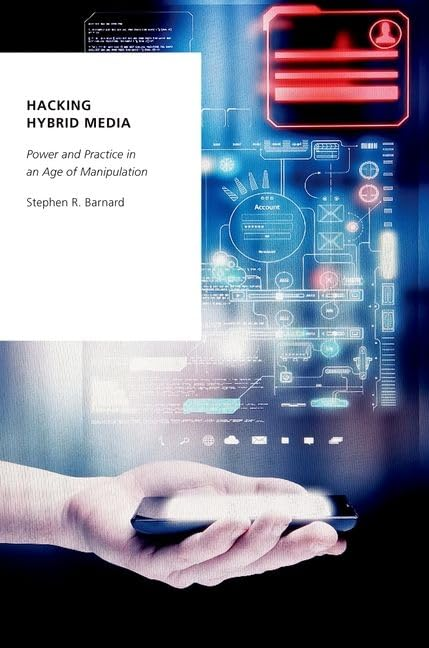
\includegraphics[width=\textwidth]{Fig1.png}
 \caption*{\fullcite{barnard2024}}
 %\caption{\fullcite{nascimento_formacao_2019}.}
 \label{fig01}
\end{minipage}
\end{figure}

Stephen Barnard é professor no domínio das Ciências da Comunicação e os seus interesses de investigação incluem as mídias, as tecnologias e as relações de poder. O seu percurso científico, ao longo do qual tem acumulado conhecimento e mobilizado teorias oriundas de vários campos, conduz a um trabalho interdisciplinar. Nos seus diversos trabalhos, tem ligado, de modo muito interessante, abordagens qualitativas e quantitativas; é especialmente o caso quando se trata da transformação digital e das suas consequências para a opinião pública, e para as instituições políticas e mediáticas. Ao longo da sua obra "Hacking Hybrid Media: Power and Practice in an Age of Manipulation", Barnard explora as potenciais disfunções do sistema mediático híbrido, ou seja, como os fundos tecnológicos e as dinâmicas culturais preparariam um terreno para a manipulação e a polarização política e informativa. No entanto, essa complexidade reflete a natureza complexa da influência das mídias. 

A obra estrutura-se através da abordagem de estudos de casos e do desenvolvimento teórico e conceptual sobre as práticas de manipulação das mídias na era digital. Em termos orgânicos, a obra é constituída por sete capítulos, refletindo sobre como os atores políticos, as plataformas digitais e a opinião pública interagem com as narrativas mediáticas circulantes.

O autor começa por introduzir o conceito de sistema mediático híbrido, caracterizando-o como uma estrutura que combina as lógicas dos meios de comunicação tradicionais e das plataformas digitais. Mais concretamente, defende que “[…] é necessário considerar estes fenómenos no contexto de um sistema mediático híbrido, uma integração de meios de comunicação mais recentes e mais antigos em que as práticas mediáticas mais recentes nos campos interpenetrados dos meios de comunicação e da política adaptam e integram as lógicas das práticas mediáticas mais antigas nesses campos e vice-versa” \cite[p. 17 tradução nossa]{barnard2024}. Essa definição é claramente devedora da ideia de crescente hibridez do sistema mediático de \textcite{chadwick2017}. Neste contexto, nas mídias tradicionais, os jornalistas e editores atuam como guardiões, controlando o fluxo informativo que chega até aos cidadãos e público em geral. Com a digitalização, essa dinâmica alterou-se radicalmente e as possibilidades oferecidas pelas plataformas digitais permitem um fluxo de informação mais descentralizado e interativo.

Um caso que serve de ilustração é a Convenção do Partido Republicano de 2019, nos Estados
Unidos, na qual Donald Trump, com a ajuda de influenciadores digitais conservadores, pôde
difundir e reforçar narrativas, muito para além dos participantes neste encontro partidário. Esse exemplo, descrito como um “pseudo-evento”, ilustra a forma como os atores políticos moldam e condicionam com sucesso o discurso público através das potencialidades tecnológicas do sistema mediático híbrido. Com efeito, Barnard introduz o conceito de “capital mediático em rede”, central na sua análise, que descreve a capacidade dos atores de utilizarem recursos tecnológicos e mediáticos para reforçarem a sua influência no debate público.

Mais, Barnard advoga que o sistema midiático híbrido não é simplesmente uma combinação de lógicas tradicionais e digitais, mas sim um ambiente transformador que redefine as relações de poder, criando oportunidades de participação dos cidadãos, mas também novos desafios institucionais confrontados pela disseminação massiva de desinformação que visa à manipulação.

No segundo capítulo, o autor tem como finalidade apresentar uma tipologia detalhada das práticas de manipulação, dividindo-as em três funções principais: criação, reforço e legitimação. A criação de desinformação (função geradora) é seguida de estratégias de disseminação (função reforçadora) e da confirmação da credibilidade dessas narrativas (função legitimadora).

O autor ressalta que as oportunidades digitais democratizaram o acesso à produção de conteúdos, permitindo que os atores individuais e coletivos façam uso dessas ferramentas para moldar a opinião pública. Contudo, essa democratização também abre espaço a práticas de manipulação. Barnard lança mão do modelo clássico de propaganda de Herman e Chomsky para demonstrar que, enquanto a manipulação tradicional era centralizada e controlada, o ambiente híbrido caracteriza-se por descentralização, amplificação por algoritmos e, muitas vezes, participação.

Nessa linha, Barnard enfatiza também que as novas possibilidades abertas pelas plataformas digitais tornam possível que as mensagens com desinformação cheguem a um público ainda mais heterogêneo, de forma rápida e eficaz. Tal fenômeno cria um ecossistema informativo em que as falsas narrativas não apenas podem proliferar, como também moldar a opinião pública de maneira contundente, redefinindo a relação entre tecnologia, conhecimento e poder. 

No terceiro capítulo, Barnard aborda as consequências da abolição da doutrina da neutralidade, nos Estados Unidos, em 1987. Essa alteração regulatória eliminou a exigência do equilíbrio na informação noticiosa. De acordo com o autor, a decisão deu espaço ao crescimento dos conteúdos polarizadores nos meios de comunicação tradicionais, como rádio e televisão, e preparou o terreno para o sensacionalismo que se verifica em boa parte do discurso midiático contemporâneo. Desse modo, com a solidificação de um modelo comunicacional fundamentado em mecanismos descentralizados, tais tendências foram exacerbadas. Os líderes políticos passaram a poder contornar facilmente os intermediários tradicionais, como jornalistas e comentaristas, e interagir diretamente com o público, utilizando plataformas digitais para apoiar narrativas possivelmente polarizadoras. De acordo com Barnard, essas transformações refletem tanto transformações tecnológicas quanto transformações culturais e institucionais, que criaram um ambiente midiático mais fragmentado e polarizado. 

Concomitantemente, o autor observa também a forma como a segmentação das audiências reforçou os consumos midiáticos. O fenômeno das “câmaras de eco” surge como uma consequência direta das lógicas algorítmicas, que dão prioridade aos conteúdos que reforçam as percepções pré-existentes dos utilizadores. Essa dinâmica não apenas agrava a polarização, mas também restringe a criação de espaços de diálogo e consenso. Assim sendo, Barnard aponta para os desafios que as mídias tradicionais enfrentam, dentro do ambiente híbrido. A diminuição da confiança nas instituições jornalísticas e a ascensão de plataformas que favorecem o engajamento em detrimento da qualidade informativa estão ameaçando a capacidade do jornalismo para desempenhar sua função social. Tal análise é crucial na elaboração para compreender os fatores estruturais que modelam o sistema midiático contemporâneo.

O quarto capítulo examina a forma como as plataformas digitais atuam como intermediários do sistema híbrido e como moldam o discurso público de uma forma que normalmente privilegia a desinformação. Segundo Barnard, as plataformas, regidas por modelos de negócio que priorizam o lucro, geram condições favoráveis à disseminação de conteúdos polarizadores e mobilizadores emocionalmente. Por exemplo, pode-se mencionar o ataque ao Capitólio, nos Estados Unidos, em 2021. O autor utiliza esse evento para ilustrar como as oportunidades tecnológicas que possibilitam as plataformas podem servir tanto à mobilização democrática como a atividades extremistas. Enfatiza que essas capacidades permitem aos grupos organizados fazer circular eficazmente falsas narrativas, frequentemente fabricando percepções enganosas que influenciam a opinião pública e o seu comportamento. 

Nessa linha de pensamento, Barnard critica a falta de transparência das plataformas digitais relativamente aos algoritmos e aos processos de moderação de conteúdos. O autor considera que a autorregulação das empresas tecnológicas não é suficiente para enfrentar os desafios da manipulação da informação e da polarização. Com efeito, o autor faz a apologia de maior regulação e de práticas mais transparentes, que responsabilizem as plataformas.

Simultaneamente, o autor reflete sobre a forma como as capacidades das plataformas tornam os conteúdos manipuladores altamente virais. Ferramentas como memes, vídeos editados e campanhas coordenadas tornam-se armas poderosas nas mãos de atores que compreendem as dinâmicas do sistema híbrido. Ao reforçarem narrativas errôneas, essas práticas põem em causa a integridade dos processos democráticos e a coesão social.

Nos capítulos cinco e seis, Barnard apresenta estudos de caso que ilustram as práticas de manipulação abordadas ao longo do livro. O primeiro exemplo é o incidente entre o jornalista da CNN Jim Acosta e uma estagiária da Casa Branca. A partir de um vídeo que havia sido objeto de manipulação, serviu de justificação para alegações de abuso por parte do jornalista. Esse caso exemplifica como os atores políticos podem se apropriar de ferramentas digitais para ajustar percepções e controlar narrativas veiculadas junto à opinião pública.

No segundo caso, o autor analisa o fórum The\_Donald, uma plataforma digital utilizada pelos apoiantes de Donald Trump para coordenar estratégias de manipulação. Os membros do fórum utilizaram técnicas como memes, tendo como finalidade a manipulação de algoritmos para promover narrativas que visam desinformar e manipular.

Barnard analisa a forma como a migração do fórum para uma plataforma independente, depois de o Reddit ter imposto restrições, intensificou as práticas extremistas. Esse exemplo é particularmente relevante para compreender como os espaços digitais alternativos podem atuar como incubadoras de práticas manipuladoras, com consequências significativas para a integridade democrática.

Esses estudos de caso ligam eficazmente as teorias a exemplos concretos, demonstrando a relevância prática da análise de Barnard e tornando o trabalho acessível tanto aos acadêmicos como ao público em geral.

No último capítulo, Barnard resume os argumentos apresentados e introduz o conceito de “dialética da (des)informação”. Defende que as práticas manipuladoras e as narrativas desinformativas criam um ciclo de retroação em que a desinformação e a polarização se reforçam mutuamente e exacerbam as desigualdades estruturais e culturais.

Em diálogo com a obra e o seu autor:

Se bem que o autor oferece soluções, como a proposta de mais transparência nas plataformas digitais, regulamentação efetiva e educação mediática, estas são feitas de forma descritiva sem especificar como elas devem ser operacionalizadas. Barnard observa que a reação ao sistema midiático híbrido deve ser coletiva, salientando que essas soluções conjuntas devem mobilizar governos, empresas de tecnologia e cidadãos.

Um contributo da obra é a defesa de uma verdadeira e efetiva política que vise incrementar o letramento midiático como ferramenta essencial para combater a manipulação da informação, tal como vários autores têm vindo a defender \cite{souza2022a}. Barnard sugere que os cidadãos devem ser capacitados através da educação para analisar criticamente os conteúdos que consomem e partilham, encorajando um envolvimento mais consciente e responsável. Essa proposta tem a limitação de se concentrar em medidas que visam indivíduos, porém há necessidade de medidas mais amplas como a inclusão em programas de formação escolar \cite{souza2023}.

O autor alerta, ainda, para os riscos associados à concentração de poder nas plataformas digitais. Argumenta que, embora as novas potencialidades tecnológicas democratizem o acesso à informação, também criam condições para a perpetuação das desigualdades de poder, uma vez que alguns atores exploram desproporcionadamente essas ferramentas, algo que tem vindo a ser reforçado por vários autores como \textcite{nielsen2022}.

\textit{Hacking Hybrid Media} é uma obra indispensável para compreender a dinâmica do poder e da manipulação no atual sistema midiático híbrido. Ao articular reflexão teórica rigorosa com estudos de caso empíricos, Barnard promove uma visão interdisciplinar e acessível sobre as práticas de manipulação na era digital.

Não obstante serem identificadas algumas limitações, como a concentração na realidade norte-americana e a falta de propostas mais pormenorizadas para resolver os problemas identificados, a obra caracteriza-se pela profundidade e relevância da reflexão que gera. Oferece não só uma crítica perspicaz, mas também um valioso ponto de partida para futuras investigações sobre a área de estudos de sobreposição entre as mídias, a política e a tecnologia.


\printbibliography\label{sec-bib}
% if the text is not in Portuguese, it might be necessary to use the code below instead to print the correct ABNT abbreviations [s.n.], [s.l.]
%\begin{portuguese}
%\printbibliography[title={Bibliography}]
%\end{portuguese}


\end{document}

